% TODO for references: when using blog-posts, thematize that academic publishing is rather slow, especially as compared to the developments in the world of web technologies.
% Meta: for claims, just start out with a TODO-marker, then if the reference actually ends up in the finished text, find a reference to support the claim.

\chapter{Suggested Solution}

% TODO RUNNING EXAMPLE
% fkleedorfer_rsa [5:25 PM] 
% vielleicht ein 'running example' im suggested solution teil?
% an dem man sehen kann was man schreiben muss, um in der architektur was einzubauen
% zb: User tippt eine message und drückt enter

% TODO REGEAR TO COMPARISON OF TOOLS AND WHEN TO CHOOSE WHAT (for similar scenarios as ours)
% FK: ist doch schon mal was.. vielleicht eine vergleichsmatrix oder längeres eingehen auf die gründe für die Wahl?

% CHAPTER-OUTLINE:
% 1. one section on tool-choices
% 1. one section on the current architecture (how we planned it vs how it turned out, e.g. actors directly accessing state)
% 1. one on future work: 
%     * drop actors, drop angular / look at ng2
%     * NOTE: The Architecture fails somewhat at keeping sync state across tabs, implementing that is a lot of effort on top of it. Theoretically we could serialize and sync the entire state (making sync a lot easier than with angular and flux), but it’s still no Falcor, Relay or Meteor(?) in that regard.

\section{Stack}

\begin{comment}

* meinkauf app -> ng-redux has good DX

components:

* bi-directional binding was causing a lot of bugs (how many?) -> less angular
* migrate -> ng-redux instead of react 
* modularity -> slightly lessened by redux. reusable components shouldn't be connected to redux but gain input via properties. most components are clearly app-specific anyway.
* seperation of conerns -> all do that, redux does it with less concepts / clearer imo
* redux reduces problems with asynchronity (the actions make app behaviour predictable / understandable / replayable -- tbh, the same would go for events on the angular root) 
* angular has problems with triggering events while a dispatch is in progress (we had problems with endless loops a few times (TODO link))

* Migration:
  * Reducing bootstrap usage.
  * Promises: \$q to native.
  * started with router and core reducers(?)
  * a lot of mocking → smooth collaboration
  * how did we migrate, step-by-step (central redux architecture first, then add components, write import wrapper for won.js, restructure linkeddata-service.js)

build tool: pure npm vs grunt vs gulp vs brunch?

* too complex for chaining commands in npm (<- is it really?)
* gulp seemed to be best practice with it's pipes (with grunt being too old and brunch not well known)
* TODO better arguments

dependencies - npm vs bower vs jspm vs yarn: 

* not all packages on npm
* bower has many gui packages but no perceivable advantage beyond that and makes the build more complex
* jspm also integrates packaging and crosscompiling and can do npm, bower and github as source
* yarn beats npm for speed and predictability but can only do npm as source (afair)

why bundle at all: no endless include lists in index.jsp anymore
module syntax - amd/requirejs/commonjs vs es6: es6 is the standardized way
bundling - browserify vs webpack vs jspm: 

css-preprocessor - less vs sass: more people (TODO numbers) and better tooling for sass. both have similiar functionality

css framework: we also switched away from bootstrap, as we'd need to modify it’s styles that heavily anyway

css code-styling - oocs vs bem: we're not trying to develop a generic style atm (though we probably could have developed against the bootstrap/semcss/tachyon list of classes). bem avoids name-clashes (due to css' global name-space) and has a focus on components. however, turns out that oocss seems to more reusable and easy to learn (link to sources of pro-oocss article)







    



\section{Research Rigor}
``Design-science research relies upon the application of rigorous methods in both the construction and evaluation of the design artifact.''
% This means applying existing foundations and methodologies, using effective metrics and formalising. Note, however, that an overemphasis on rigor can often lead to lower relevance (Lee 1999), as many environments and artifacts defy an excessive formalism (see ``wicked problems'' at footnote \ref{ref:wicked}). %TODO better reference / use glossary entry

requirements:

• Create and post new needs. Currently these consist of a simple data-structure with a subject, textual description and optional tags or location information.
• View needs and all data in them in a human-friendly fashion
• Share links to posts with other people
• Immediately get notified of and see matches, incoming requests and chat messages
• Send and accept contact/connection requests
• Write and send chat messages

• good DX (TODO define)
• Needs to be able to keep data in sync between browser-tabs running the JS-client and the Java-based server. This happens through a REST-API and websockets.  Most messages arrive at the WoN-Owner-Server from the WoN-Node and just get forwarded to the client via the websocket. The only data directly stored on and fetched from the Owner-Server are the account details, which needs belong to an account, its key-pair and information on which events have been seen.
• As subject of a research-project, the protocols can change at any time. Doing so
should only cause minimal refactoring in the owner-application.
• In the future different means of interactions between needs – i.e. types need-to-need connections – will be added. Doing so should only cause minimal changes in the application.
• Ultimately the interface for authoring needs should support a wide range of ontolo- gies respectively any ontology people might want to use for descriptions. Adapting the authoring guys or even just adding a few form input widgets should be seamless and only require a few local changes.
• We didn’t want to deal with the additional hurdles/constraints of designing the prototype for mobile-screens at first, but a later adaption/port was to be expected.  Changing the client application for that should require minimal effort.





## Process

<!--
Flo: "I think it's interesting to describe the actual process, but you should not over-emphasize it. In the end, you came up with a design and an implementation, and that is the artifact you produced.

If you can show multiple iterations of your artifact with 'experiments' evaluating its appropriateness and refinements, fine - but don't zoom into the microscopic level (first I read this, then that, ...).

"

**argument:** feasibility wasn't clear to begin with!!! -> it's research

-->

1. peacemems notifies me of react
2. reading that, i also stumbled across flux
  * flux-article talks about problems with angular/bi-directional data-bindings resonates (same problems when debugging prev prototype) (?)
3. meinkauf app -> design by ulf(?), testing ionic (for mobile) and ng-redux. DX is good (TODO define DX)
4. new ulf screens for won-app → we’ll need to rewrite (?)
4. rewriting with the old angular setup (angular 2 isn’t production ready)
4. pre-compilation (js, scss) and bundling setup
  * we also switched away from bootstrap, as we'd need to modify it’s styles that heavily anyway
4. actually: when stores and synching via the ws became a thing, started researching flux, ended up stumbling across redux (#342)
  * apparently, we were using flux even before that (see #342). it’s part of a commit from 23 Sep 2015 (1395ba6) and was only used to test with a draft store, so nvm.
  * and compared different implementations ( 	b824aa2)
6. read up on redux and ways to integrate with existing code-base
7. implementation
  * Frankangular - the Migration Process. Reducing angular to a rendering stage.
  * Frankangular - Duplicate imports :{
  * Migration:
      * Reducing bootstrap usage.
      * Promises: $q to native.
   * started with router and core reducers(?)
   * a lot of mocking → smooth collaboration
8. usability tests (?) not really part of architecture

* Meta: möglichst so, dass ich nichts mehr machen soll
* Meta: Write in a way that large parts can be used as WoN-documentation(?)
* Meta: always spell in full first names of female authors for references
* Meta: repeat important points with different wordings.

The Architecture fails somewhat at keeping sync state across tabs, implementing that is a lot of effort on top of it. Theoretically we could serialize and sync the entire state (making sync a lot easier than with angular and flux), but it’s still no Falcor, Relay or Meteor(?) in that regard.

“iteratively identifying deficiencies in prototypes and creatively developing solutions to address them” (Markus et al., 2002)

es6-includes make bundling a lot easier (no endless include lists in index.jsp anymore)

how did we migrate, step-by-step (central redux architecture first, then add components, write import wrapper for won.js, restructure linkeddata-service.js)

medium.js text field

rdfstore-js:

* use it for caching but not as redux store
* accessing it is asynch (reducers are synchronous)
* not all app data is described in rdf

compare with other architectures (angular 1.X, flux, cyclejs’ mvi, elm,...)

how did co-workers deal with it? ease of use?

interaction/integration with project mngmt workflows. e.g. pull-requests, mocking,...

more difficult architectural decisions:

* Routing
* Rdf-store
* Access Management


## Relevant Github-Issues

* [Owner App README](https://github.com/researchstudio-sat/webofneeds/tree/master/webofneeds/won-owner-webapp) basically describes our redux setup
* [The New Code Base Structure - Structure Diagrams, Refactoring and more](https://github.com/researchstudio-sat/webofneeds/issues/151) (#151)
* [Map widget](https://github.com/researchstudio-sat/webofneeds/issues/222)  (#222) and [marker clustering](https://github.com/researchstudio-sat/webofneeds/issues/227) (#227)
  * leafletjs and osm
* [Address forms](https://github.com/researchstudio-sat/webofneeds/issues/226) (#226)
* [Password-retyping unnecessary if reset-via-email works](https://github.com/researchstudio-sat/webofneeds/issues/264) (#264)
* Experiences with contenteditable ([#278](https://github.com/researchstudio-sat/webofneeds/issues/278))
* [Angular 2.0](https://github.com/researchstudio-sat/webofneeds/issues/300) (#300)
* [Precompilation and Tooling (Bundling, CSS, ES6)](https://github.com/researchstudio-sat/webofneeds/issues/314) (#314)
  * bundling, svg sprites, sass, es6,�  - why and how?
  * SASS and BEM. Also address Semantic CSS (!)
* [SVG-sprites](https://github.com/researchstudio-sat/webofneeds/issues/318) (#318)
* [Template Parsing Performance](https://github.com/researchstudio-sat/webofneeds/issues/319) (#319) - jsx
* [Speech-Bubble-CSS](https://github.com/researchstudio-sat/webofneeds/issues/333) (#333)
  * Afair we now use a better version by simply rotating a div with a border.
* [Documentation-generator](https://github.com/researchstudio-sat/webofneeds/issues/337) (#337)
* [Actions/Stores and Synching ](https://github.com/researchstudio-sat/webofneeds/issues/342) (#342)
  * meta: figures in issue need updates
  * this is the issue that triggered the redux research.
  * Redux ~ Elm Architecture ~ CycleJS Model-View-Intent. The parts (Action-Creators / Actions, Reducers, Views). Insights on handling side-effects (e.g. server-side interaction)
  * dealing with rdf-store
* [Routing and Redux](https://github.com/researchstudio-sat/webofneeds/issues/344) (#344)
* [chrome’s security](https://github.com/researchstudio-sat/webofneeds/issues/372) (#372)
* [WebSocket only created before login](https://github.com/researchstudio-sat/webofneeds/issues/381) (#381)
* [Direct link to need](https://github.com/researchstudio-sat/webofneeds/issues/517).
* [nicer urls via html5mode in ui-router](https://github.com/researchstudio-sat/webofneeds/issues/520) (#520)
* [Speed up build](https://github.com/researchstudio-sat/webofneeds/issues/577) (#577) aka "`jspm install` is slow when you need to run it on every build"
* [Page-load performance optimisation](https://github.com/researchstudio-sat/webofneeds/issues/546) (#546)
* [Human-friendly timestamps ](https://github.com/researchstudio-sat/webofneeds/issues/549) (#549) → tick actions
* [Load data selectively](https://github.com/researchstudio-sat/webofneeds/issues/623) (#623) – Paging
* [Flatten content-node of needs](https://github.com/researchstudio-sat/webofneeds/issues/719) (#719)
* [direct link to conversation not working](https://github.com/researchstudio-sat/webofneeds/issues/728) (#728)
* Unify Directives: Overview » Incoming Requests and Matches List
* Unify Directives: Chat and Incoming Request and Outgoing Request
* [Usability Tests of Demonstrator](https://github.com/researchstudio-sat/webofneeds/issues/752) (#752)

\end{comment}




















\section{Architecture}\label{architecture}
\todo{Reword so it fits into the thesis. Change all links to github issues
to point to other sections of the thesis.}

We're using the redux-architecture for the won-owner-webapp javascript-client.
The architecture is strongly based on
\fnurl{http://redux.js.org/}{redux} in general and
\fnurl{https://github.com/wbuchwalter/ng-redux}{ng-redux} in particular. You can
find a short overview over these and their actions, reducers, the store and components
in section \ref{ref:redux}. For more in-depth
and hands-on documentation beyond what has been used for the work preceding
this thesis, I can recommend reading their well-done documentations.

So, this section will document in what ways our architecture diverges from or
builds on top of basic (ng-)redux, as well as list experiences and
style-recommendations from using it. %TODO these latter points should be in the critical reflection section

\begin{figure*}
\centering
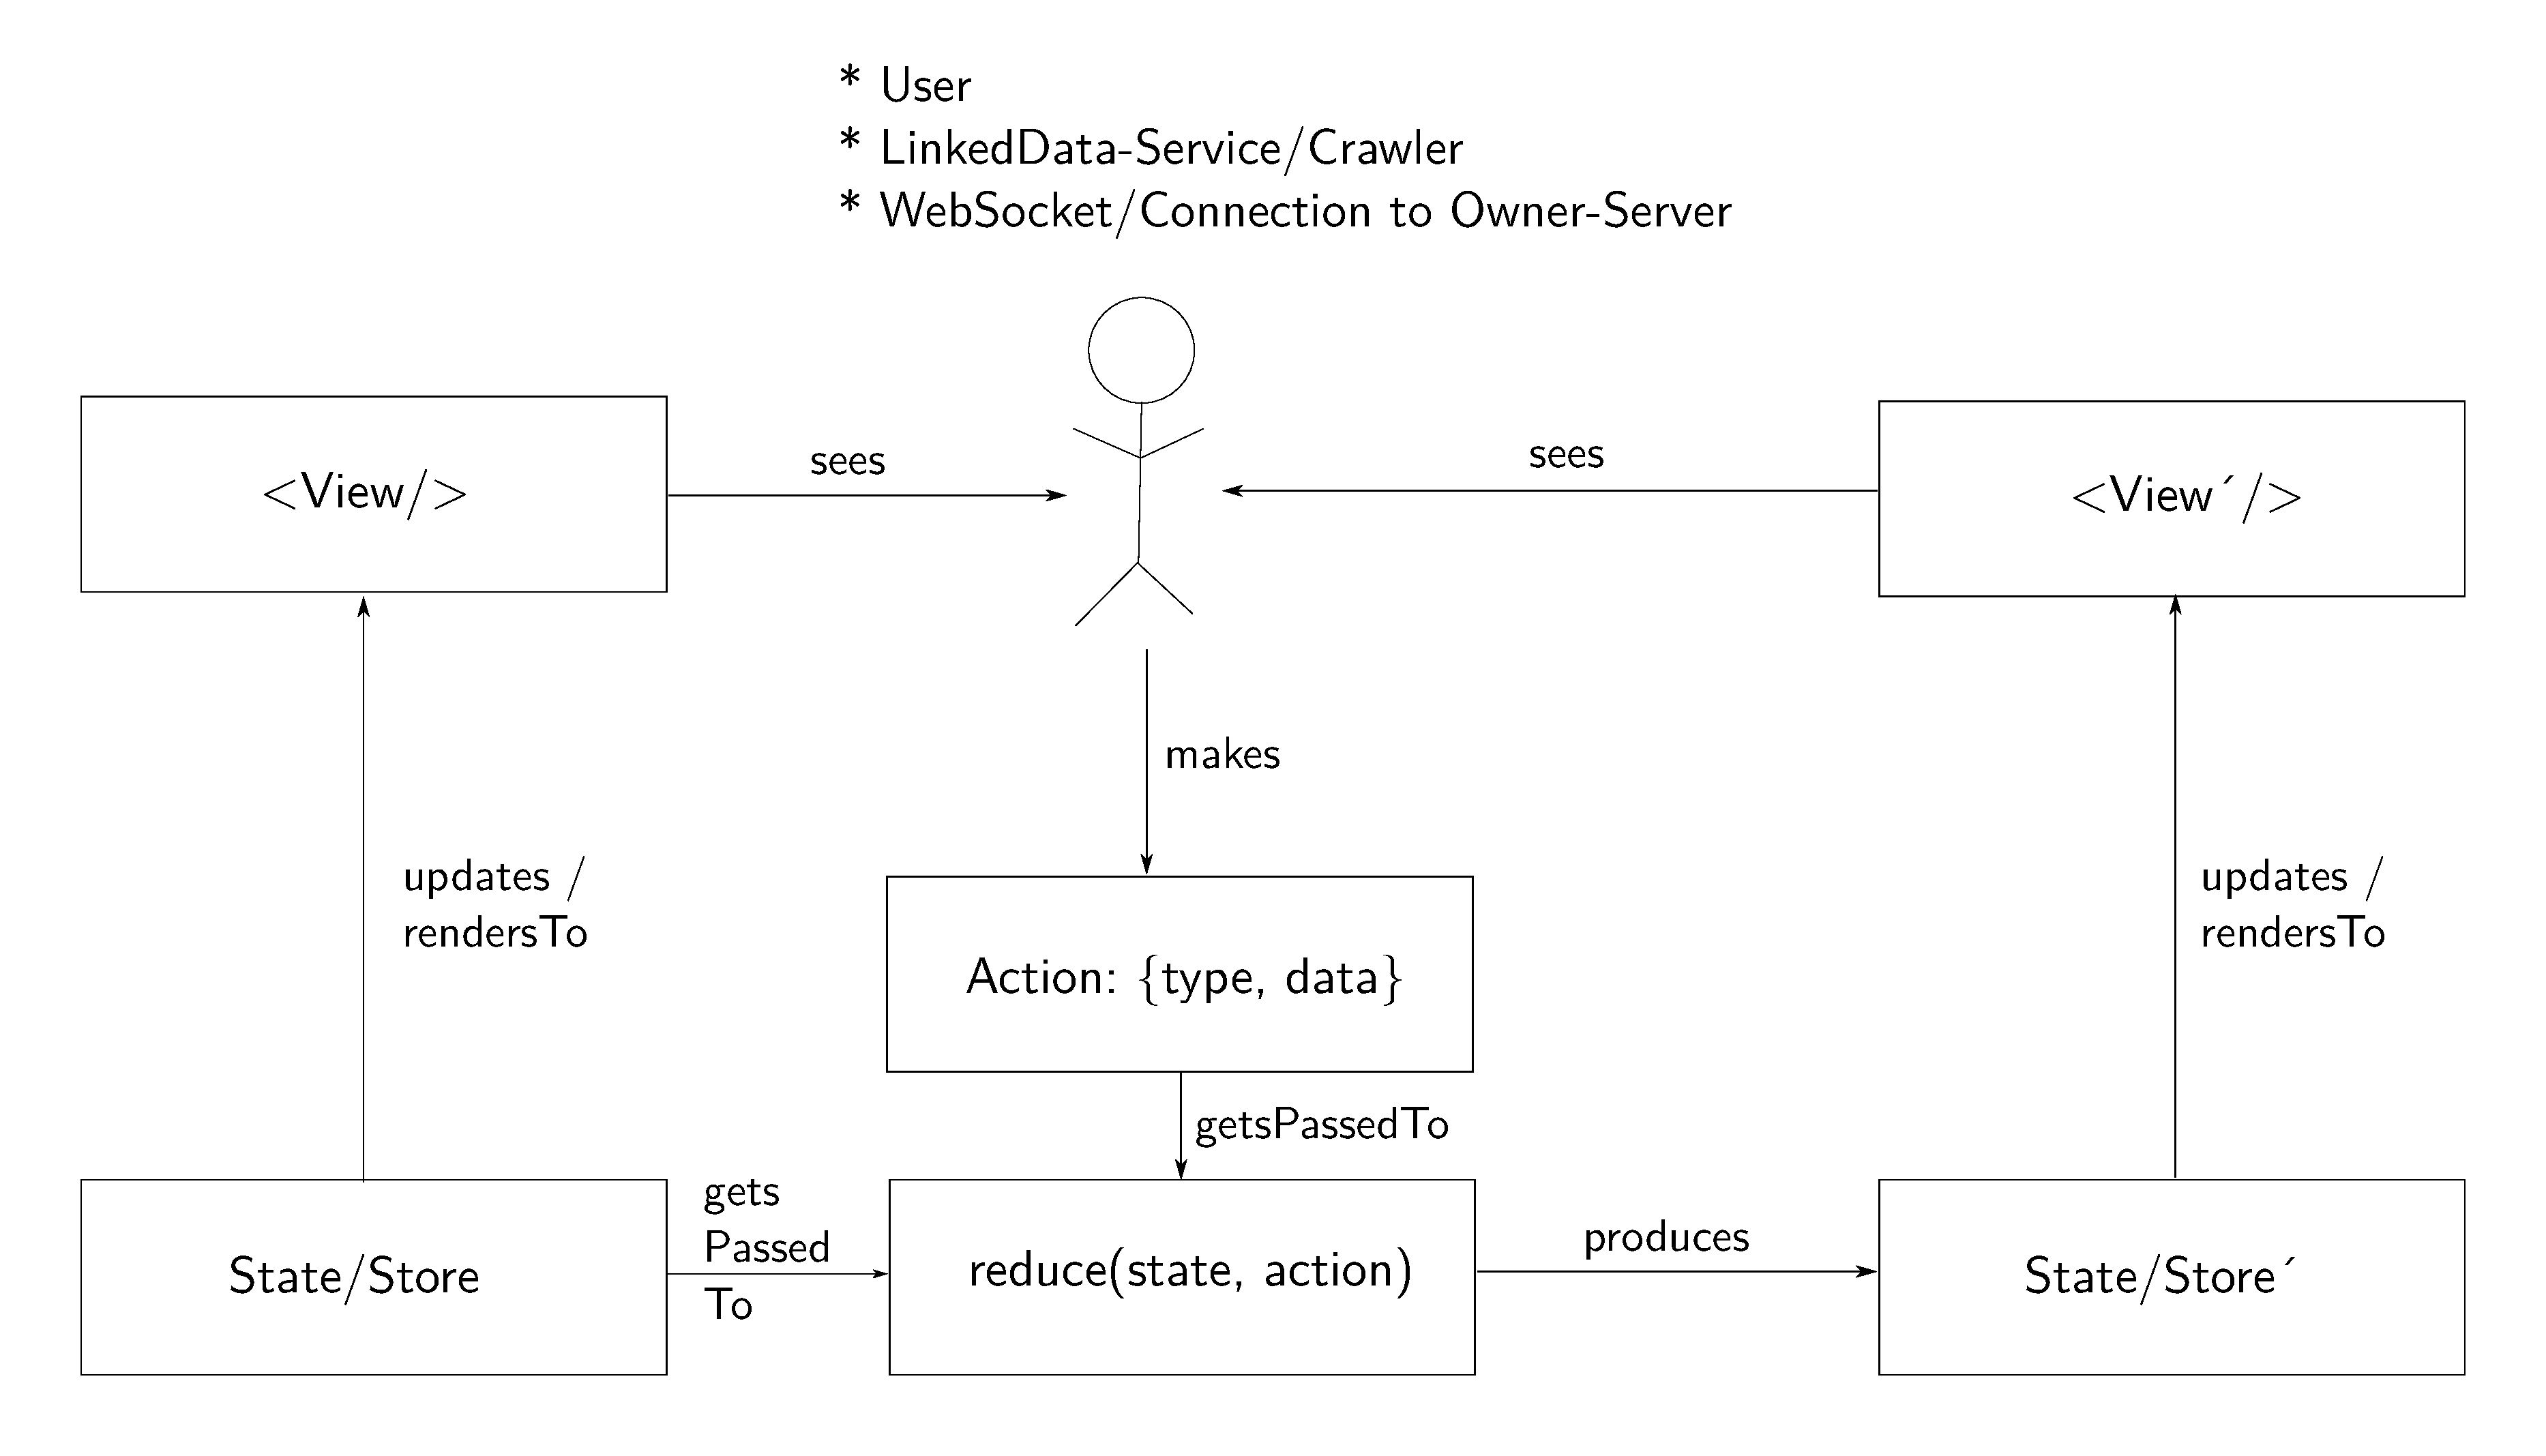
\includegraphics[width=1.0\textwidth]{figures/owner_app_redux_architecture.pdf}
\caption{\label{fig:adapted-redux}redux architecture in client-side owner-app}
\end{figure*}

\subsection{Action Creators}\label{sct:action-creators}

Can be found in \texttt{app/actions/actions.js} % TODO put into apendix

Anything that can cause \textbf{side-effects} or is
\textbf{asynchronous} should happen in these (tough they can also
be synchronous -- see \texttt{INJ\_DEFAULT}) %TODO code snippet
They should only be triggered
by either the user or a push from the server via the
\texttt{messagingAgent.js}. In both cases they cause a
\textbf{single}(!) action to be dispatched and thus passed as
input to the reducer-function.

If you want to \textbf{add new action-creators} do so by adding to the
\texttt{actionHierarchy}-object in \texttt{actions.js}. % TODO reword. this thesis isn't for colleagues working on the same code-base
From that two objects are generated at the moment:

\begin{itemize}
\tightlist
\item
  \texttt{actionTypes}, which contains string-constants

  (e.g.
  \texttt{actionTypes.drafts.change.title\ ===\
  \textquotesingle{}drafts.change.title\textquotesingle{}})
\item
  \texttt{actionCreators}, which houses the action creators. for the
  sake of injecting them with ng-redux, they are organised with
  \texttt{\_\_} as seperator (e.g.

  \texttt{actionCreators.drafts\_\_change\_\_title(\textquotesingle{}some\ title\textquotesingle{})})
\end{itemize}

Btw, the easiest way for actions without sideffects is to just placing
an \texttt{myAction:\ INJ\_DEFAULT}. This results in an action-creator
that just dispatches all function-arguments as payload, i.e.
\texttt{actionCreators.myAction\ =\ argument\ =\textgreater{}\ (\{type:\ \textquotesingle{}myAction\textquotesingle{},\ payload:\ argument\})}

Actions and their creators should always be describe \textbf{high-level user
stories/interactions} like \texttt{matches.receivedNew} or \texttt{publishPost}
(as opposed to something like \texttt{matches.add}
or \texttt{data.set})
Action-creators
encapsule all sideeffectful computation, as opposed to the reducers
which (within the limits of javascript) are guaranteed to be
side-effect-free. Thus we should do \textbf{as much as possible within
the reducers}. This decreases the suprise-factor/coupling/bug-proneness
of our code and increases its maintainability.

\subsection{Actions}\label{actions}

Can be found in \texttt{app/reducers/reducers.js} % TODO put into appendix

They are objects like
\texttt{\{type:\ \textquotesingle{}drafts.change.title\textquotesingle{},\ payload:\ \textquotesingle{}some\ title\textquotesingle{}\}}
and serve as input for the reducers.

See:
\href{https://github.com/researchstudio-sat/webofneeds/issues/342}{Actions/Stores
and Synching} %TODO should be in-thesis ref

\subsection{Reducers}\label{reducers}

Can be found in \texttt{app/reducers/reducers.js} % TODO put into appendix

These are \textbf{side-effect-free}. Thus as much of the implementation
as possible should be here instead of in the action-creators
to profit from this guarantee and steer clear of possible sources for
bugs that are hard to track down.

See ``Action Creators'' in section \ref{sct:action-creators} above for more detail

\subsection{Components}\label{components}

They live in \texttt{app/components/}. % TODO put into appendix?

Top-level components (views in the angular-sense) have their own folders
(e.g. \texttt{app/components/create-need/} and are split in two files).
You'll need to add them to the routing (see below) to be able to switch
the routing-state to these.

Non-top-level components are implemented as directives.

In both cases open up the latest implemented component and use the
boilerplate from these, if you want to implement your own. Once a
refined/stable boilerplate version has emerged, it should be documented
here.

\subsection{Routing}\label{routing}

We use
\href{https://github.com/angular-ui/ui-router/wiki/Quick-Reference}{ui-router}
and in particular the
\href{https://github.com/neilff/redux-ui-router}{redux-wrapper for it}
%TODO make thesis-intern

Routing(-states, aka URLs) are configured in \texttt{configRouting.js}. %TODO put into appendix
State changes can be triggered via
\texttt{actionCreators.router\_\_stateGo(stateName)}. % TODO too code-docu-like
The current
routing-state and -parameters can be found in our app-state:

\begin{verbatim}
$ngRedux.getState().get('router')
/* =>
{
  currentParams: {...},
  currentState: {...},
  prevParams: {...},
  prevState: {...}
}
*/
\end{verbatim}

Also see:
\href{https://github.com/researchstudio-sat/webofneeds/issues/344}{Routing
and Redux} %TODO make thesis-intern

\subsection{Server-Interaction}\label{server-interaction}

If it's \textbf{REST}-style, just use
\texttt{fetch(...).then(...dispatch...)} in an action-creator.
%TODO reword and elaborate

If it's \textbf{linked-data-related}, use the utilities in
\texttt{linkeddata-service-won.js}. They'll do standard HTTP(S) but will
make sure to cache as much as possible via the local triplestore.
%TODO reword and elaborate

If needs to \textbf{push to the web-socket}, add a hook for the
respective \emph{user(!)}-action in \texttt{message-reducers.js}. The
\texttt{messaging-agent.js} will pick up any messages in
\texttt{\$ngRedux.getState().getIn({[\textquotesingle{}messages\textquotesingle{},
\textquotesingle{}enqueued\textquotesingle{}  ]})}
and push them to it's websocket. This solution appears rather hacky to
me (see `high-level interactions' under `Action Creators') and I'd be
thrilled to hear any alternative solutions :)
%TODO reword and elaborate

If you want to \textbf{receive from the web-socket}, go to
\texttt{actions.js} and add your handlers to the
\texttt{messages\_\_messageReceived}-actioncreator. The same I said
about pushing to the web-socket also holds here.
%TODO reword and elaborate 
\section{Tooling}\label{tooling}

\begin{comment}

* bundling
* css
* es6


\begin{itemize}
\tightlist
\item
  \href{https://github.com/researchstudio-sat/webofneeds/issues/300}{Angular
  2.0} -\textgreater{} it wasn't ready at the time of the decision
\item
  \href{https://github.com/researchstudio-sat/webofneeds/issues/314}{Precompilation
  and Tooling (Bundling, CSS, ES6)}
\end{itemize}
\end{comment}


